%
%
%

\begin{frame}[t]{Perceptron}

    The \index{perceptron}\Gls{perceptron} 
    is the simplest \index{neural network}neural network.

    It contains a single input layer and an output node.

    \begin{center}
        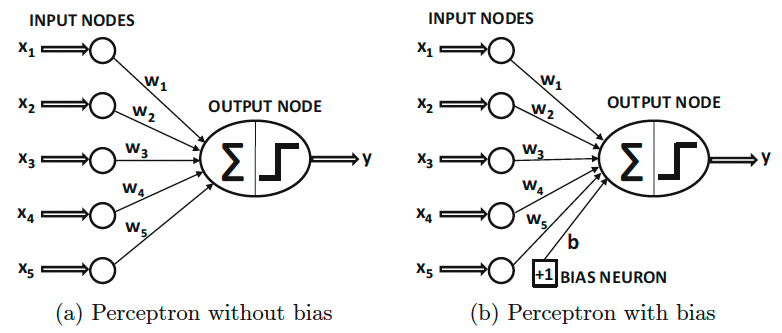
\includegraphics[width=0.85\textwidth]{./images/perceptron/basic_architecture.png}\\
        {\scriptsize \color{col:attribution} 
        Basic architecture of the perceptron. 
        Image reproduced from p.5 of \cite{Aggarwal:2018SpringerDL}}\\
    \end{center}

    It is a 
    \index{binary classification}binary classification 
    algorithm for 
    \index{supervised learning}supervised learning.

\end{frame}

%
%
%

\begin{frame}[t]{What problem does the perceptron tries to solve?}

    Consider the following problem. You have:
    \begin{itemize}
        \item a {\bf vector of $d$ feature variables}, $\vect{x}$ = $(x_1, x_2, ..., x_d)^T$, and
        \item a {\bf single binary variable} $y$ ($\in$ \{-1, +1\}).   
    \end{itemize}
    The binary variable $y$ \underline{depends on} the feature variables $\vect{x}$.\\
    \vspace{0.2cm}

    \begin{blockexample}{}
    \begin{itemize}
        \small
        \item 
        $\vect{x}$ may describe observed properties of a tumor imaged 
        using computed tomography (CT) scan and 
        $y$ may describe whether the tumor is benign or malignant,
        \item 
        $\vect{x}$ may characterize energy depositions and geometrical features of 
        an event observed in a particle physics detector and 
        $y$ may describe whether the event is a new physics candidate 
        or conventional Standard Model background,
        \item 
        $\vect{x}$ may include details about a credit card transaction, such
        as time, amount, location, and frequency of past transactions, and 
        $y$ may describe whether the transaction is fraudulent or not.
    \end{itemize}
\end{blockexample}

\end{frame}

%
%
%

\begin{frame}[t]{What problem does the perceptron tries to solve?}

    Consider the following problem. You have:
    \begin{itemize}
        \item a {\bf vector of $d$ feature variables}, $\vect{x}$ = $(x_1, x_2, ..., x_d)^T$, and
        \item a {\bf single binary variable} $y$ ($\in$ \{-1, +1\}).   
    \end{itemize}
    The binary variable $y$ \underline{depends on} the feature variables $\vect{x}$.\\
    \vspace{0.2cm}
    

\end{frame}

%
%
%

\begin{frame}[t]{Perceptron}

    \begin{columns}
        \begin{column}{0.50\textwidth}
         \begin{center}
          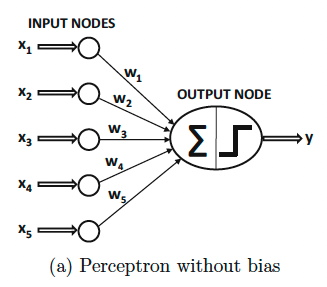
\includegraphics[width=0.98\textwidth]{./images/perceptron/perceptron_without_bias.png}\\
          \vspace{0.5cm}
          {\scriptsize \color{col:attribution} 
          Basic architecture of the perceptron. 
          Image reproduced from p.5 of \cite{Aggarwal:2018SpringerDL}}\\
         \end{center}
        \end{column}
        \begin{column}{0.50\textwidth}
            \begin{equation}
                \hat{y} = sign\Big\{ \vect{w}^T \cdot \vect{x} \Big\} = sign\Big\{ \sum_{i=1}^{d} w_i x_i \Big\}
             \end{equation}        
        \end{column}
      \end{columns}
      
\end{frame}

%
%
%

\begin{frame}[t]{Perceptron}

    \begin{columns}
        \begin{column}{0.50\textwidth}
         \begin{center}
            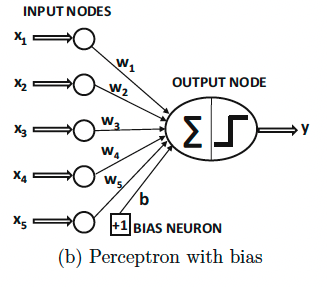
\includegraphics[width=0.98\textwidth]{./images/perceptron/perceptron_with_bias.png}\\
            \vspace{0.5cm}
            {\scriptsize \color{col:attribution} 
            Basic architecture of the perceptron. 
            Image reproduced from p.5 of \cite{Aggarwal:2018SpringerDL}}\\
         \end{center}
        \end{column}
        \begin{column}{0.50\textwidth}
            \begin{equation}
                \hat{y} = 
                    sign\Big\{ \vect{w}^T \cdot \vect{x} \Big\} = 
                    sign\Big\{ \sum_{i=1}^{d} w_i x_i + b \Big\}
             \end{equation}
            The bias can be incorporated as the weight of an additional ($d$+1) feature 
            variable that always takes the value of 1.        
        \end{column}
      \end{columns}

\end{frame}

%
%
%

\begin{frame}[t]{Perceptron}

    \begin{equation}
        L = \sum_{(\vect{x},y) \in D} (y - \hat{y})^2 
          = \sum_{(\vect{x},y) \in D} \Bigg(y - sign\Big\{ \vect{w}^T \cdot \vect{x} \Big\}\Bigg)
     \end{equation}


\end{frame}

%
%
%

\begin{frame}[t]{Perceptron}

\end{frame}

%
%
%

\begin{frame}[t]{Perceptron}

\end{frame}

%
%
%

\begin{frame}[t]{Perceptron}

\end{frame}
